\documentclass[tikz]{standalone}
\usetikzlibrary{intersections}
\begin{document}
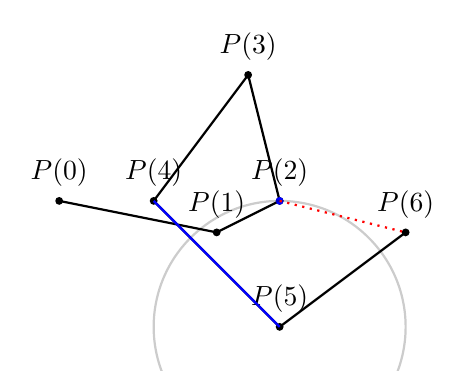
\begin{tikzpicture}[scale=0.4]
  \useasboundingbox (-1,5.5) rectangle (12,-4.5);
  \foreach \i/\x/\y in {0/0/0, 1/5/-1, 2/7/0, 3/6/4, 4/3/0, 5/7/-4, 6/11/-1}{
    \coordinate (p\i) at (\x, \y);
    \node[circle,fill,color=black,inner sep=1pt,label={[text=black, above]:\(P(\i)\)}] at (p\i) [] {}; 
  }
  \foreach \i in {0,...,5}{
    \pgfmathsetmacro{\next}{\i+1}
    \draw[thick] (p\i) -- (p\next);
  }

  \node[circle,fill,color=blue,inner sep=1pt] at (p2) [] {}; 
  \draw[thick, opacity=0.2] (p5) circle (4);
  \draw[color=red, dotted, thick] (p2) -- (p6);
  \draw[color=blue, thick] (p4) -- (p5);
\end{tikzpicture}
\end{document}
